\chapter{Etude technique}

\section*{Introduction}
La conception et la modélisation sont à la base du projet. Les connaître nous permettra de bien définir les autres composantes et besoins de ce projet. Cela comprend les choix techniques et les outils informatiques utilisés pour obtenir des résultats satisfaisants. C'est un projet  structuré avec des composants interconnectés pour un excellent flux de travail.

\section{Conception et modelisation}
Maintenant que nous avons décrit les phases du problème, concentrons-nous sur les phases fondamentales du cycle de vie du logiciel: les phases de conception et de modélisation. Le but de cette phase est de dériver une spécification pour l'architecture du système. 
Cette phase conduit à la conception et à la schématisation de classes et de séquences basées sur le langage de modélisation UML.

Dans tout ce qui précède, nous pouvons remarquer une structure légèrement différente de celle que nous avons déjà montrée dans la section \ref{Solution_prop}.
    \subsection{Structure générale du projet}
    Pour construire une nouvelle structure, il faut s'appuyer sur les points issus du chapitre précédent.

    Pour ce faire, on doit utiliser une base de données secondaire. Il s'agit d'une grande base de données structurée de la population adulte, pour construire des modéles pré-entraînés sur des donnéees de la population adulte, Un phénomène décidément très proche du nôtre.
    Après tous ces considérations on a trouver la structure du figure \ref{fig:structure_gen}
    \begin{figure}[H]
        \centering
        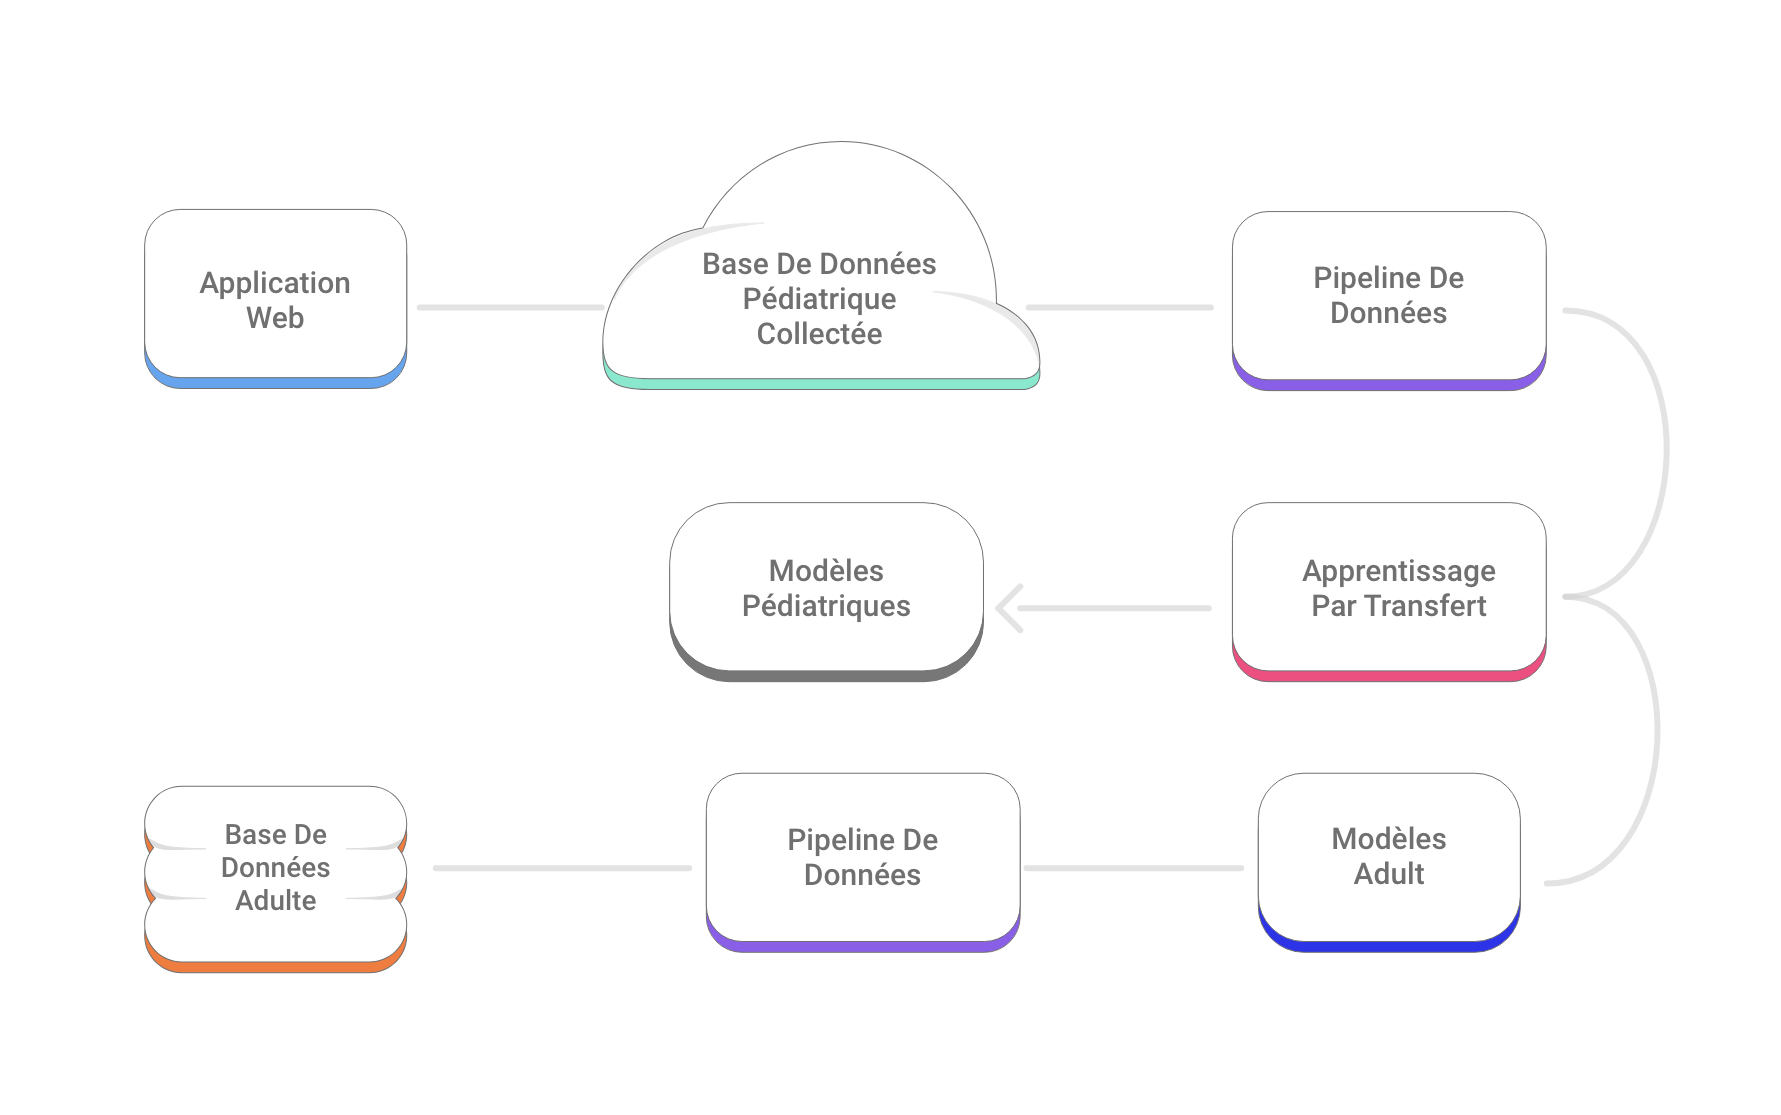
\includegraphics[width=0.7\textwidth]{structure_gen.jpg}
        \caption{structure génerale du projet}\label{fig:structure_gen}
    \end{figure}
    \subsection{Application Web}
        L'application Web est une API simple pour la collection et la visualisation de données, donc son architecture de base est également simple, c'est comme suit figure \ref{fig:xpedia_arc}
        \begin{figure}[H]
            \centering
            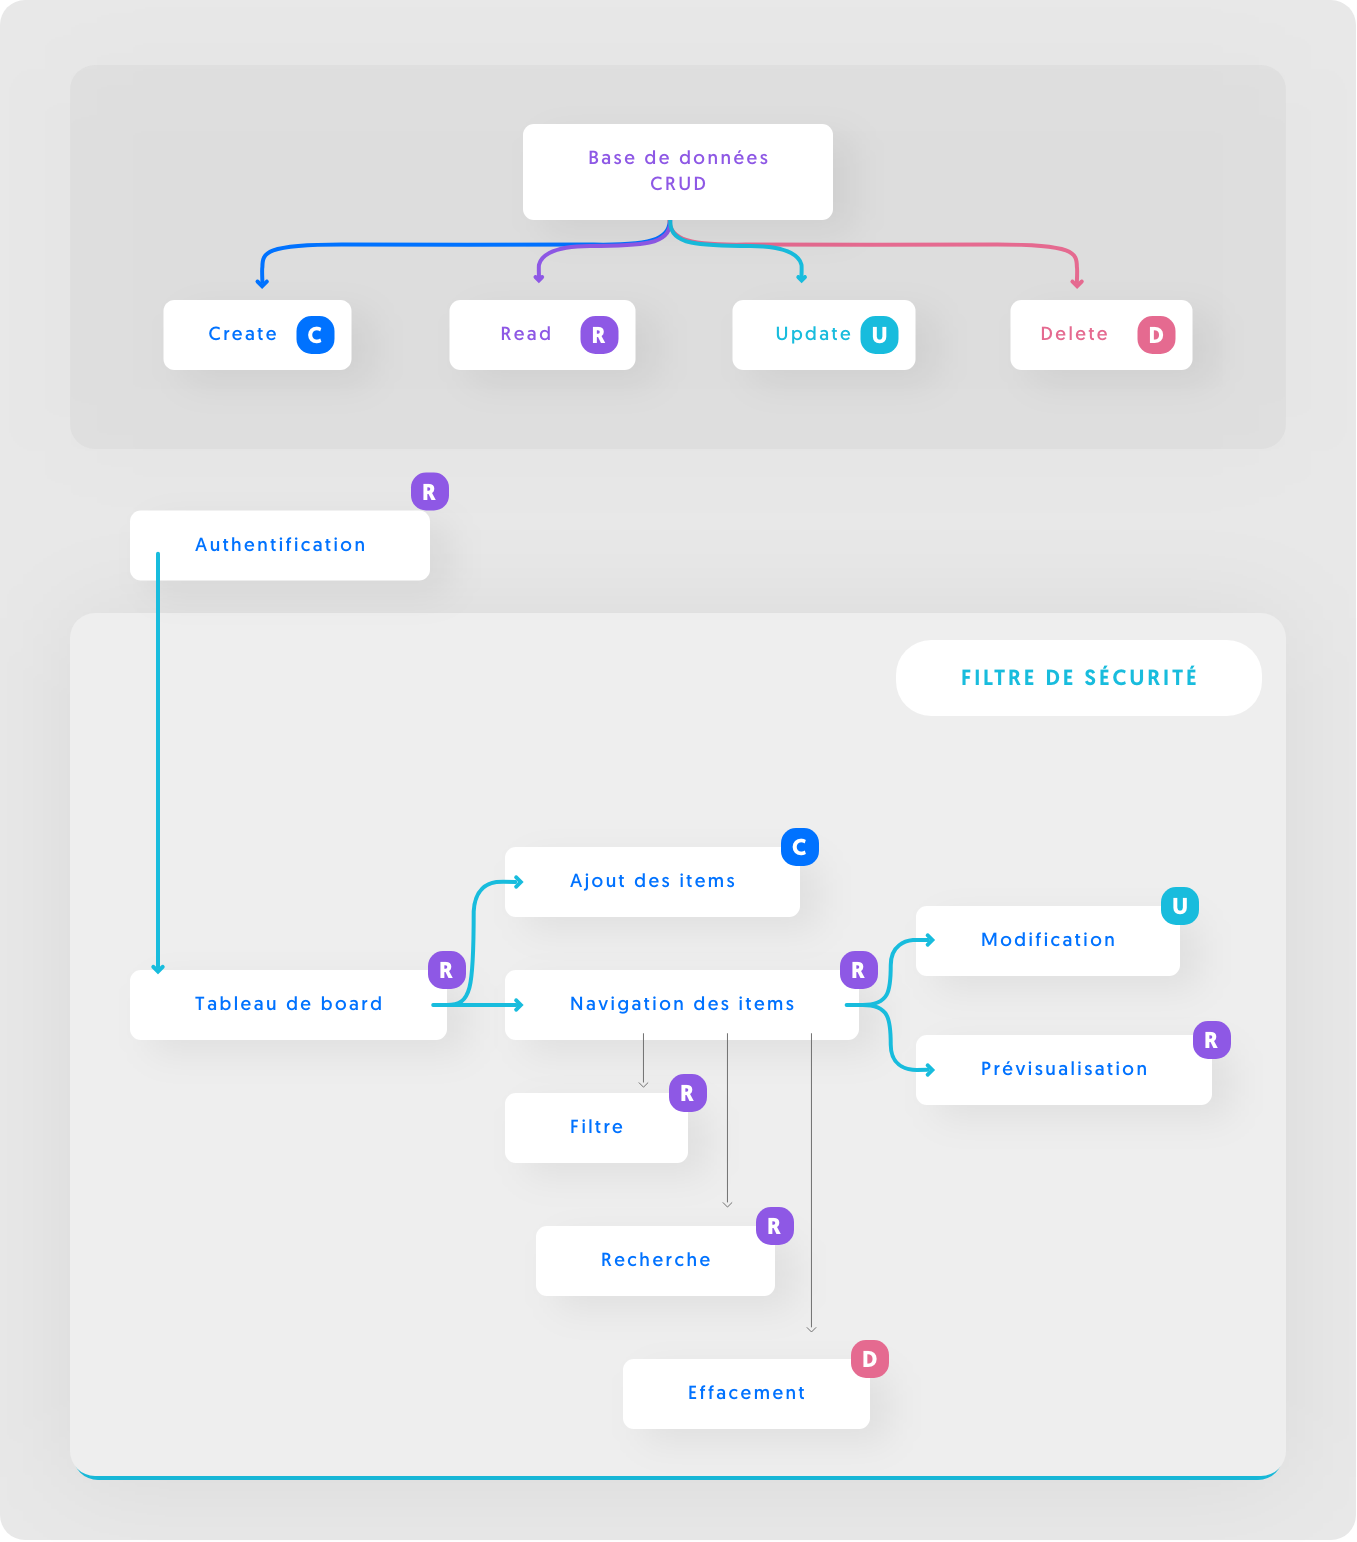
\includegraphics[width=1\textwidth]{xpedia_arc.png}
            \caption{structure génerale de l'application web Xpedia}\label{fig:xpedia_arc}
        \end{figure}
        \subsubsection{UML}
            UML (abréviation de Unified Modeling Language) est un langage de modélisation standardisé composé d'un ensemble de diagrammes intégrés qui aident les développeurs de systèmes et de logiciels à spécifier, visualiser et visualiser les artefacts des systèmes logiciels. .système. UML représente un ensemble éprouvé de meilleures pratiques techniques pour la modélisation de systèmes vastes et complexes et constitue une partie très importante du développement logiciel orienté objet et du processus de développement logiciel. UML utilise principalement une notation graphique pour représenter la conception de projets logiciels.

            \begin{enumerate}
                \item Diagramme de classe:
                Notre diagramme de classe de  deux classes utilisateur et xray (cliché), notre but de cette application et de collectés les données (xrays), l'acteur qui va effectuer la collection est l'utilisateur:
                \begin{figure}[H]
                    \centering
                    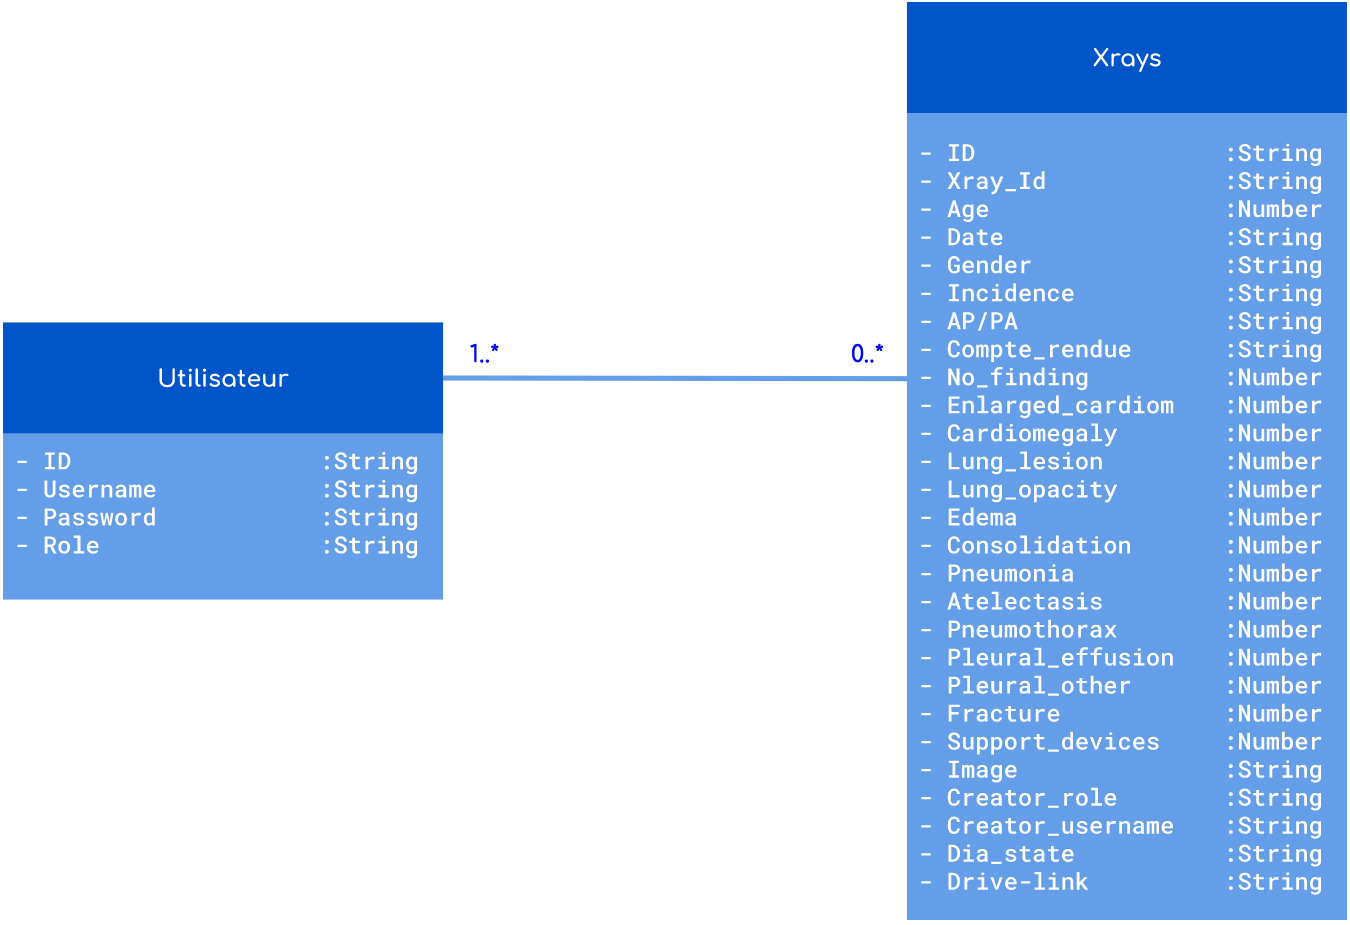
\includegraphics[width=0.8\textwidth]{class_dia.png}
                    \caption{Le diagramme de classe de l'application web Xpedia}\label{fig:class_dia}
                \end{figure}

                \item Diagrammes de séquence
                
                Un diagramme de séquence représente les objets impliqués dans une interaction particulière et les messages qu'ils échangent organisés par ordre chronologique.
                \begin{enumerate}
                    \item Diagramme de séquence: cas d'authentification
                    \begin{figure}[H]
                        \centering
                        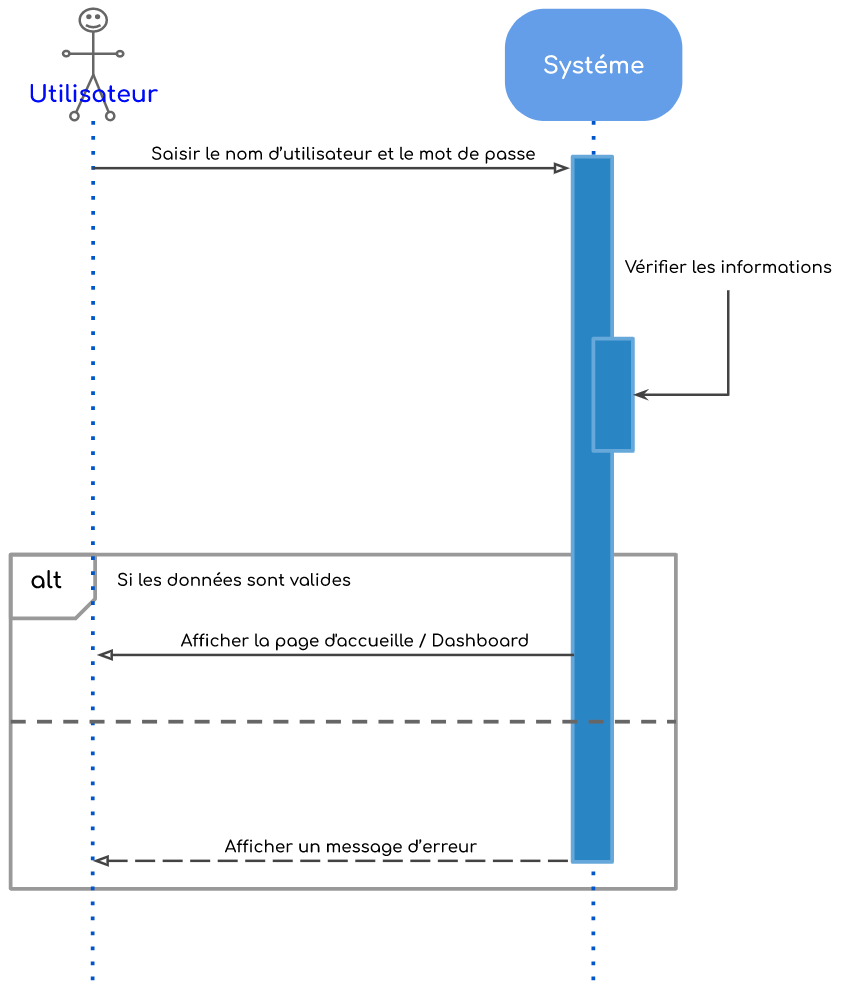
\includegraphics[width=0.5\textwidth]{cas_auth.png}
                        \caption{Le diagramme de séquence: cas d'authentification}\label{fig:cas_auth}
                    \end{figure}

                    Comme on peut le voir sur la figure \ref{fig:cas_auth}, l'authentification se fait à travers 2 opérations principales:
                    \begin{itemize}[label=$\bullet$]
                        \item l'utilisateur fournit le nom d'utilisateur et le mot de passe
                        \item le système recoupe les informations fournies avec les données existantes dans la collection de l'utilisateur
                    \end{itemize}
                    \item Diagramme de séquence: cas d'ajouter un cliché
                    \begin{figure}[H]
                        \centering
                        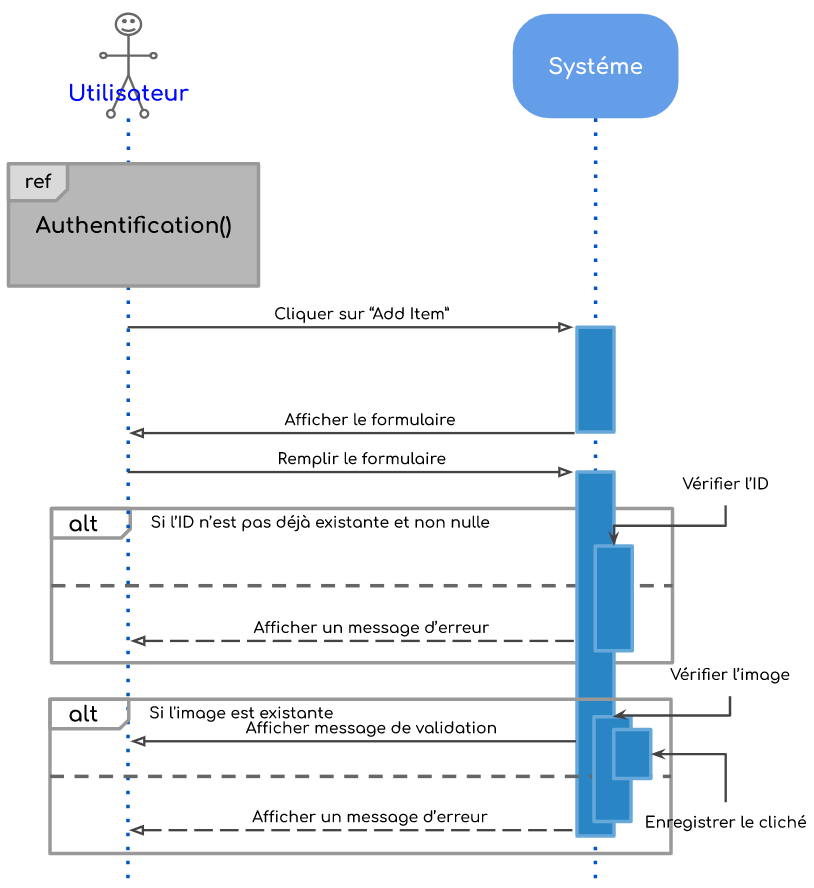
\includegraphics[width=0.5\textwidth]{cas_add.png}
                        \caption{Le diagramme de séquence: cas d'ajouter un cliché}\label{fig:cas_add}
                    \end{figure}
                \end{enumerate}
            \end{enumerate}
        
    \subsection{Pipeline de données}
    \paragraph*{Un pipeline de données est} une série d'étapes de traitement de données. Si les données ne sont pas actuellement chargées dans la plateforme de données, elles seront ingérées au début du pipeline. Ensuite, vous avez une séquence d'étapes où chaque étape fournit une sortie qui devient l'entrée de l'étape suivante. Cela continue jusqu'à ce que le pipeline soit terminé. Dans certains cas, des étapes indépendantes peuvent s'exécuter en parallèle.  
    
    Un pipeline de donnéesse compose de trois éléments principaux : une source, une ou plusieurs étapes de traitement et une destination. Dans certains pipelines de données, une destination peut être appelée un récepteur. Par exemple, un pipeline de données peut transmettre des données de votre application à un entrepôt de données, d'un lac de données à une base de données d'analyse ou à un système de traitement des paiements. Un pipeline de données peut également avoir la même source et le même récepteur, de sorte que le pipeline n'a besoin que de modifier l'ensemble de données. Chaque fois que des données sont traitées entre le point A et le point B (ou les points B, C, D), il existe un pipeline de données entre ces points.
    \begin{figure}[H]
        \centering
        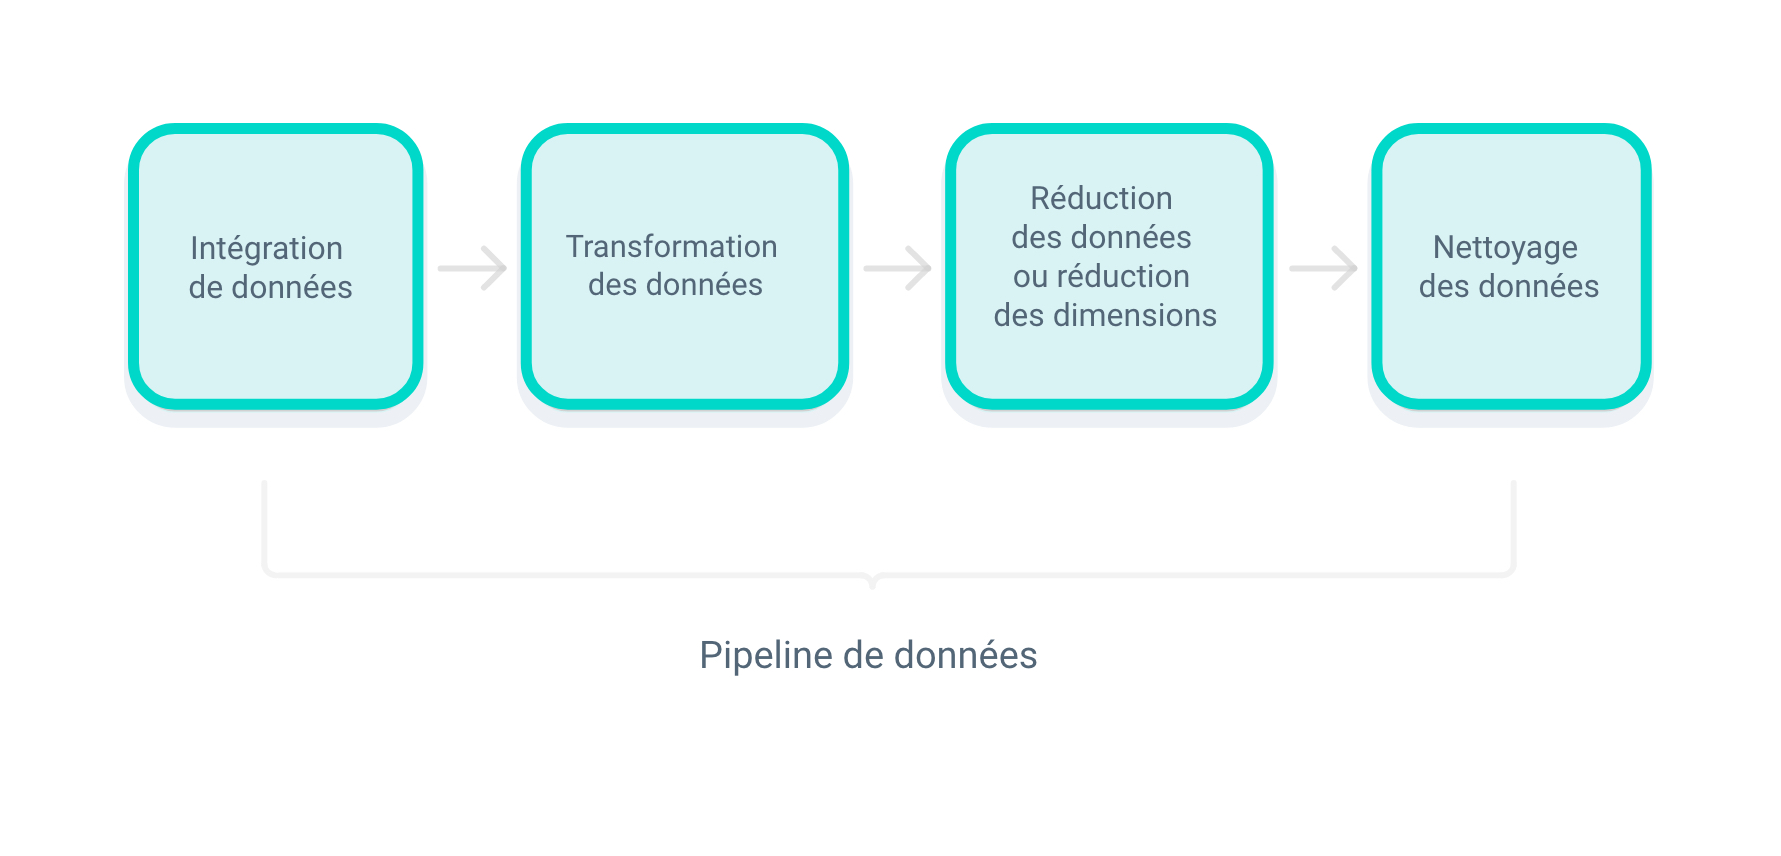
\includegraphics[width=0.8\textwidth]{data-preprocessing.jpg}
        \caption{La structure d'un pipeline de données}\label{fig:data_preprocessing}
    \end{figure}
        \subsubsection{Integration}
        L'intégration de données est le processus consistant à combiner des données provenant de différentes sources en une vue unique et unifiée. L'intégration commence par le processus d'ingestion et comprend des étapes telles que le nettoyage, le mappage ETL et la transformation. L'intégration des données permet finalement aux outils d'analyse de produire une intelligence économique efficace et exploitable.

        Il n'existe pas d'approche universelle de l'intégration des données. Cependant, les solutions d'intégration de données impliquent généralement quelques éléments communs, notamment un réseau de sources de données, un serveur maître et des clients accédant aux données à partir du serveur maître.

        Dans un processus d'intégration de données typique, le client envoie une demande de données au serveur maître. Le serveur maître reçoit ensuite les données nécessaires à partir de sources internes et externes. Les données sont extraites des sources, puis consolidées en un seul ensemble de données cohérent. Ceci est renvoyé au client pour utilisation.
        \subsubsection{Transformation}
        La transformation des données est le processus de transformation des données d'un format à un autre. Généralement, vous convertissez du format du système source au format requis par le système cible. Les transformations de  données font partie de la plupart des tâches d'intégration et de gestion des données, telles que : B. Gestion des données et stockage des données. 

        En tant qu'étape du processus ELT/ETL, la transformation des données peut être qualifiée de « simple » ou de « complexe » selon le type de modifications qui doivent être apportées aux données avant qu'elles ne soient livrées à leur destination. Le processus de transformation des données peut être effectué à l'aide de l'automatisation, de l'administration manuelle ou d'une combinaison des deux.

        \subsubsection{Réduction}
        La réduction des données signifie la réduction de certains aspects des données, généralement le volume de données. La réduction peut également porter sur d'autres aspects tels que la dimensionnalité des données lorsque les données sont multidimensionnelles. La réduction de tout aspect des données implique généralement une réduction du volume de données.

        La réduction des données n'a de sens en soi que si elle est associée à une certaine finalité. Le but à son tour dicte les exigences pour les techniques de réduction de données correspondantes. Un but naïf de la réduction des données est de réduire l'espace de stockage. Cela nécessite une technique pour compresser les données dans un format plus compact et également pour restaurer les données d'origine lorsque les données doivent être examinées. De nos jours, l'espace de stockage n'est peut-être pas la principale préoccupation et les besoins de réduction des données proviennent fréquemment des applications de base de données. Dans ce cas, le but de la réduction des données est d'économiser le coût de calcul ou le coût d'accès au disque dans le traitement des requêtes.
        \subsubsection{Nettoyage}
        Le nettoyage des données est le processus de réparation ou de suppression des données incorrectes, corrompues, mal formées, en double ou incomplètes dans un ensemble de données. La combinaison de plusieurs sources de données augmente le risque de dupliquer ou de mal étiqueter les données. Si les données sont erronées, même si elles semblent correctes, les résultats et les algorithmes ne seront pas fiables. Il n'existe aucun moyen absolu de dicter les étapes exactes du processus de nettoyage des données, car le processus est différent pour chaque ensemble de données. Cependant, il est important de définir un modèle pour votre processus de nettoyage des données et de vous assurer que vous le faites correctement à chaque fois.


   
    \subsection{Modèles de deeplearning}

    \begin{figure}[H]
        \centering
        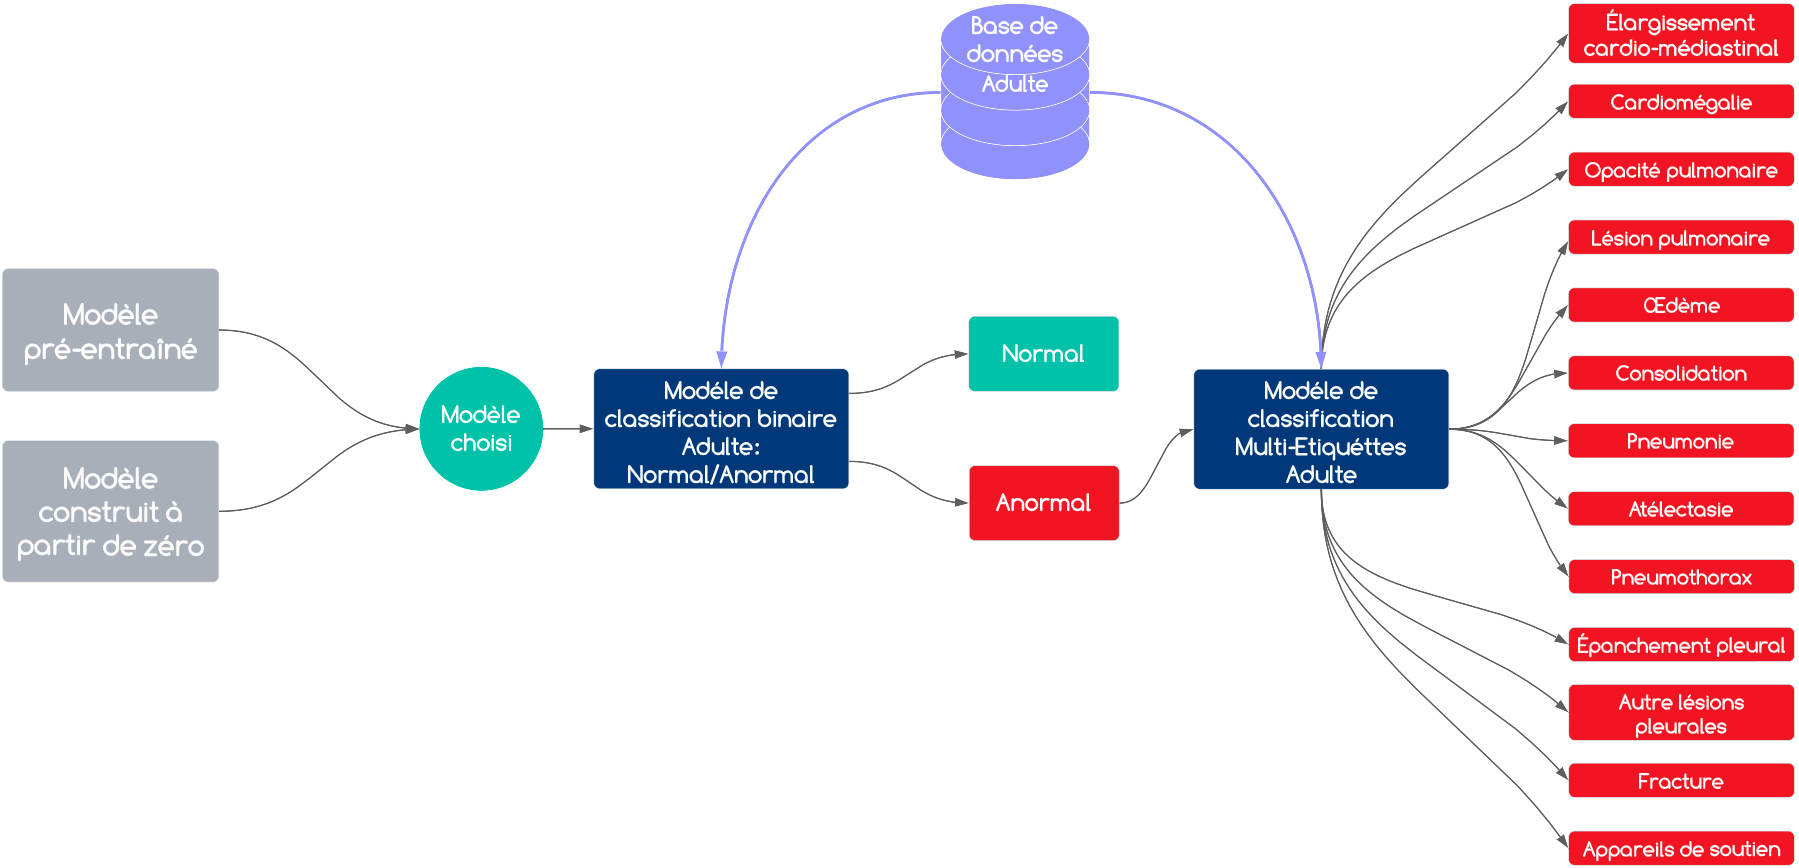
\includegraphics[width=1\textwidth]{adulte_model_train.png}
        \caption{La schéma de créeation du modèle des radiographies adultes}\label{fig:adulte_model_schema}
    \end{figure}
    \begin{figure}[H]
        \centering
        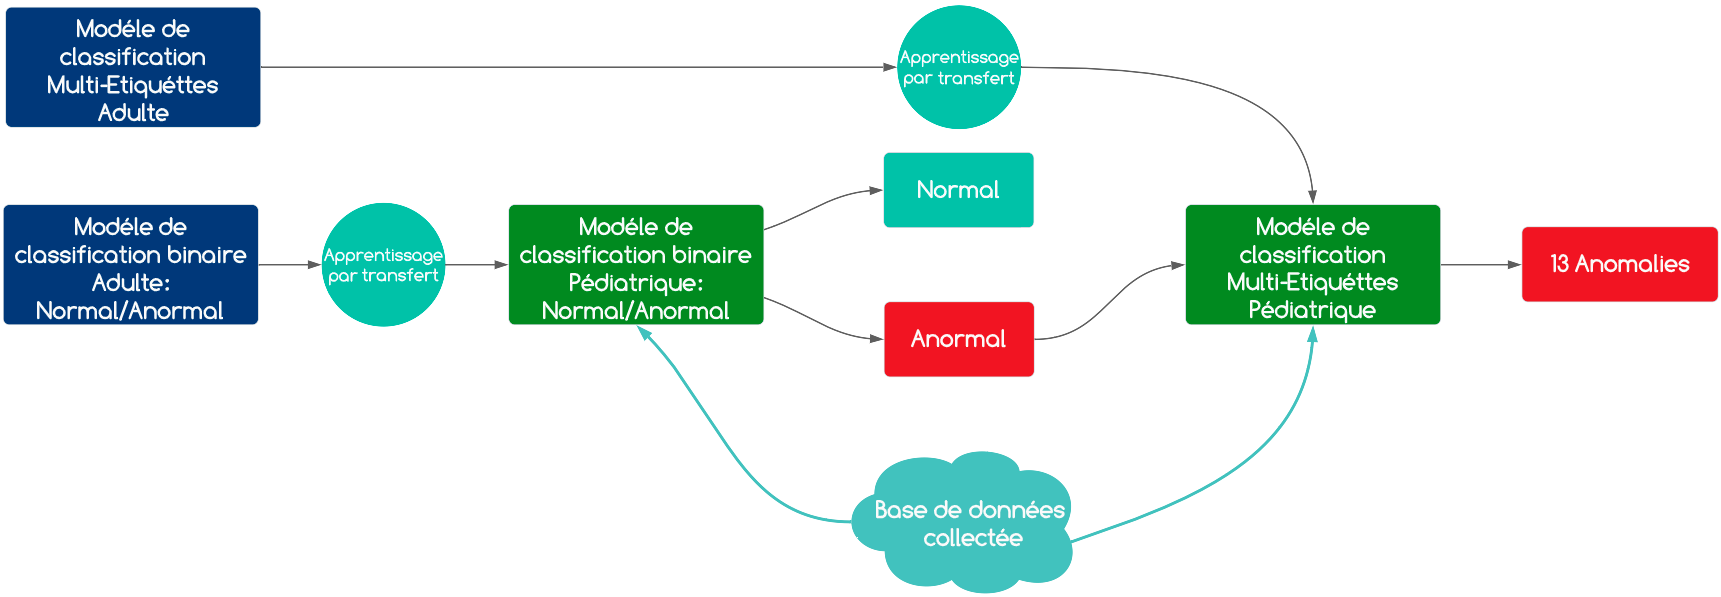
\includegraphics[width=1\textwidth]{pedia_model_train.png}
        \caption{La schéma de créeation du modèle des radiographies adultes}\label{fig:pedia_model_schema}
    \end{figure}
\section{Choix techniques}
Cette partie est consacrée à la présentation de l'environnement matériel et logiciel utilisé pour développer la solution proposée. Expliquer les décisions techniques concernant les langages de programmation et les outils à utiliser.
    \subsection{Architecture logicielle}
    \subsection{API}
    API signifie Application Programming Interface. En termes simples, une API est un ensemble de fonctions et de procédures qui vous permettent de créer une application. Accéder aux données et fonctionnalités d'autres applications, services ou systèmes d'exploitation. 
    Vous êtes essentiellement un intermédiaire entre différentes plates-formes logicielles. Ils permettent à deux applications indépendantes de "parler" entre elles. 
    Par exemple, supposons que vous êtes un agent de change fortement impliqué dans les marchés financiers et le trading. L'API peut lier un ensemble d'algorithmes de trading automatisés à la plateforme de courtage de trading préférée d'un trader. Il permet aux traders de visualiser les cotations et les données de prix en temps réel, ainsi que d'effectuer des transactions électroniques.

    \begin{figure}[H]
        \centering
        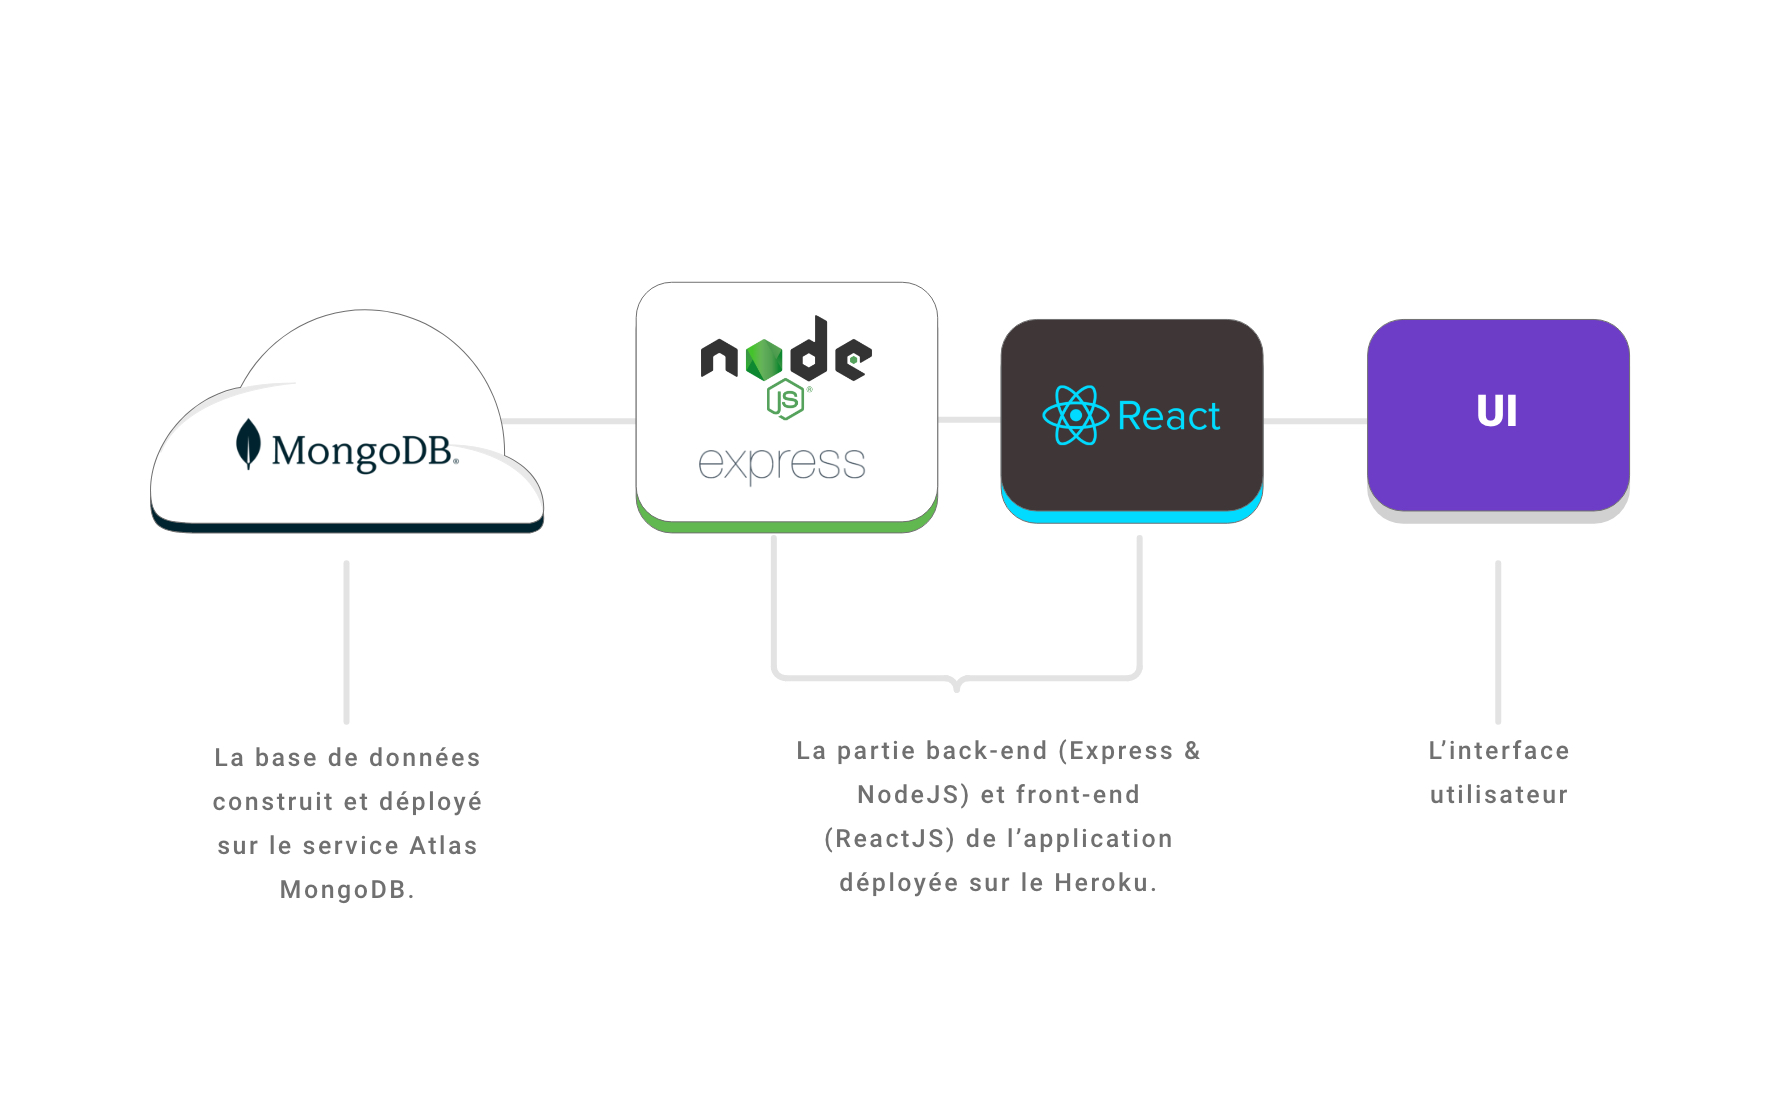
\includegraphics[width=1\textwidth]{log_arc.jpg}
        \caption{La schéma de logicielle de l'application web Xpedia}\label{fig:log_arc}
    \end{figure}

    \subsubsection{MERN stack}
    \begin{figure}[H]
        \centering
        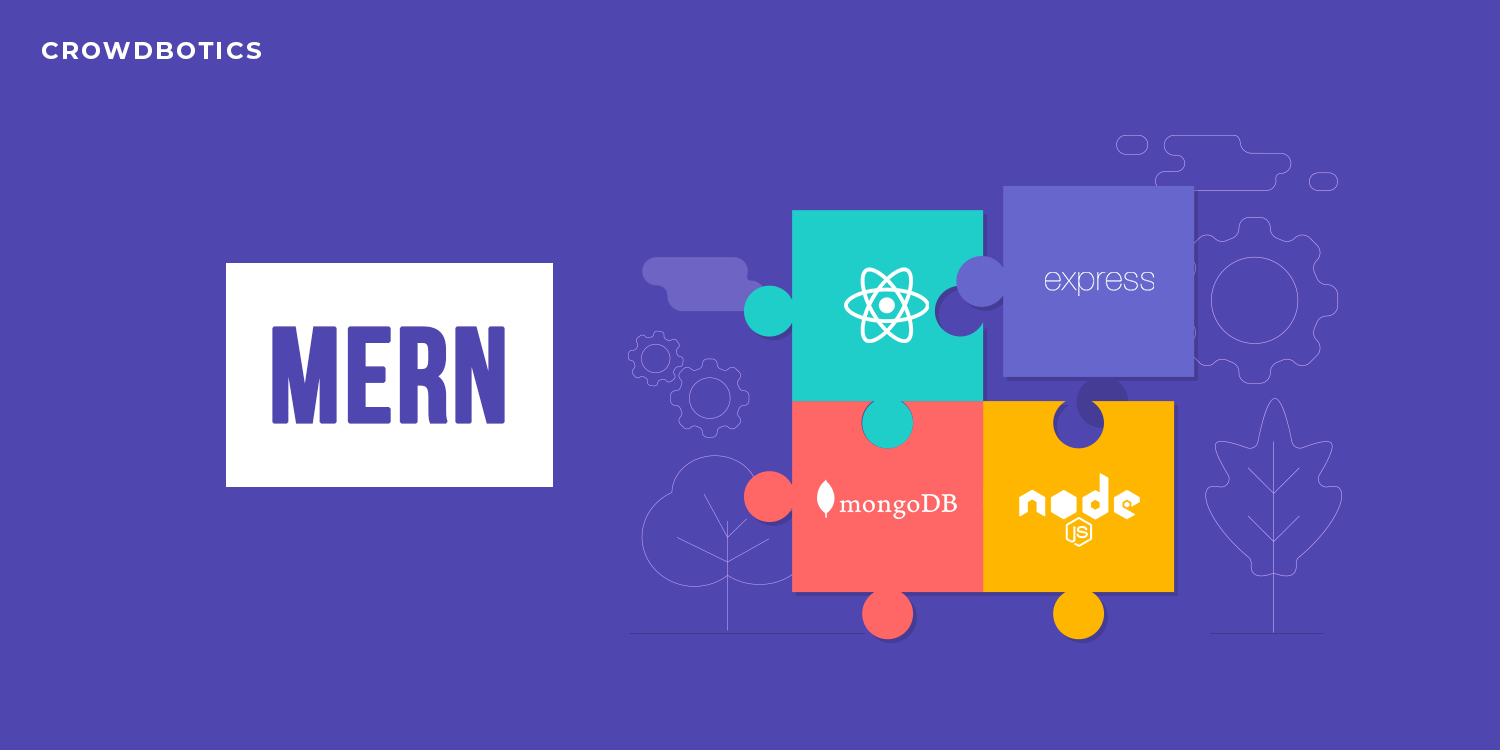
\includegraphics[width=0.6\textwidth, trim={5cm, 3cm, 5cm, 5cm},clip]{MERN.png}
        \caption{Le logo du MERN stack}\label{fig:mern}
    \end{figure}
    \paragraph{MERN Stack} est un ensemble de technologies puissantes et fiables utilisées pour développer des applications informatiques évolutives qui incluent des composants back-end, front-end et de base de données. JavaScript est utilisé pour développer des sites Web entiers plus rapidement et plus facilement.

    C'est une technologie qui est un framework JavaScript complet et convivial pour la création d'applications et de sites Web dynamiques.

    \paragraph{Pour quoi MERN?}MERN stack séparé en deux composants: le back-end et le front-end. De plus, l'ensemble du système de base de données est isolé du reste.

    L'ensemble du système, y compris le front-end, le back-end et la base de données, utilise l'API REST, qui agit comme un "middleware" et est réutilisable pour toute autre application: logiciel mobile, etc., très facilement.

    L'API REST vous permet de connecter des applications entre elles comme les pièces d'un puzzle. Les API REST sont basées sur HTTP et imitent les styles de communication Web, ce qui les rend très avantageuses à utiliser dans MERN.
    \begin{enumerate}\bfseries
        \item Atlas MongoDB\newline
        \begin{figure}[H]
            \centering
            
\includegraphics[width=0.6\textwidth]{atlass_mdb.png}
            \caption{Logo de Atlas MongoDB}\label{fig:atlass_mdb}
        \end{figure}
        \normalfont
        MongoDB Atlas est une plateforme de données de développeur multi-cloud. Au cœur se trouve notre base de données cloud entièrement gérée pour les applications modernes. Atlas est le meilleur moyen d'exécuter MongoDB, la principale base de données non relationnelle. Le modèle de document de MongoDB est le moyen le plus rapide d'innover car les documents correspondent directement aux objets de votre code. En conséquence, ils sont beaucoup plus faciles et plus naturels à travailler. Vous pouvez stocker des données de n'importe quelle structure et modifier votre schéma à tout moment lorsque vous ajoutez de nouvelles fonctionnalités à vos applications.

        Atlas Database est disponible dans plus de 80 régions sur AWS, Google Cloud et Azure. Vous pouvez même tirer parti des déploiements multi-cloud et multi-régions, ce qui vous permet de cibler les fournisseurs et les régions qui servent le mieux vos utilisateurs. Une automatisation de pointe et des pratiques éprouvées garantissent la disponibilité, l'évolutivité et la conformité aux normes de sécurité et de confidentialité des données les plus exigeantes.
        \bfseries
        \item Express Node js\newline
        \begin{figure}[H]
            \centering
            
\includegraphics[width=0.6\textwidth]{react.png}
            \caption{Logo de ReactJS}\label{fig:react}
        \end{figure}
        \normalfont
        Express est un cadre d'application Web Node.js minimal et flexible qui fournit un ensemble  de fonctionnalités robustes pour les applications Web et mobiles. 
        Express fournit une fine couche de fonctionnalités d'application Web de base sans masquer les fonctionnalités familières de Node.js.
        \bfseries
        \item React\newline
        \begin{figure}[H]
            \centering
            
\includegraphics[width=0.6\textwidth]{react.png}
            \caption{Logo de ReactJS}\label{fig:react}
        \end{figure}
        \normalfont
        React est une bibliothèque JavaScript pour créer des interfaces utilisateur. 

        Déclaratif: React facilite la création d'interfaces utilisateur interactives. Concevez une vue simple pour chaque état de votre application et React mettra à jour et affichera efficacement le composant approprié à mesure que les  données changent. Une vue déclarative rend votre code plus prévisible, plus facile à comprendre et plus facile à déboguer. 
 
        Basé sur les composants: créez des composants encapsulés qui gèrent leur propre état et combinez-les pour créer des interfaces utilisateur complexes. Étant donné que la logique des composants est écrite en JavaScript au lieu de modèles, vous pouvez facilement transmettre de grandes quantités de données  via votre application et conserver l'état en dehors du DOM.
 
        Apprenez une fois, écrivez n'importe où: nous ne faisons aucune hypothèse sur le reste de la pile technologique, vous pouvez donc développer de nouvelles fonctionnalités dans React sans réécrire le code existant. React peut également utiliser Node pour le rendu sur le serveur  et React Native pour exécuter des applications mobiles.

        \bfseries
    \end{enumerate}
    \subsubsection{Heroku}
    \begin{figure}[H]
        \centering
        
\includegraphics[width=0.6\textwidth]{heroku.png}
        \caption{Logo de Heroku}\label{fig:heroku}
    \end{figure}

    Heroku est une plate-forme de services cloud qui a gagné en popularité  ces dernières années. Heroku est si facile à utiliser qu'il est devenu le choix incontournable pour de nombreux projets de développement. 
    L'accent mis sur la prise en charge des applications centrées sur le client facilite le développement et le déploiement  des applications. Les entreprises utilisant Heroku peuvent se concentrer sur le perfectionnement de leurs applications, tandis que la plateforme Heroku gère le matériel et les serveurs. Ce n'est pas l'infrastructure qui les soutient.

    \subsubsection{Visual Studio Code}
    \begin{figure}[H]
        \centering
        
\includegraphics[width=0.6\textwidth]{vscode.png}
        \caption{Logo de Visual Studio Code}\label{fig:vscode}
    \end{figure}
    Visual Studio Code est un éditeur de code source léger mais puissant qui s'exécute sur votre bureau et est disponible sur Windows, macOS et Linux. Il offre un support intégré pour JavaScript, TypeScript et Node.js, et dispose d'un riche écosystème d'extensions pour d'autres langages et runtimes (C, C\#, Java, Python, PHP, Go, dotNET, etc.).

    Visual Studio Code combine la simplicité d'un éditeur de code source avec de puissants outils de développement comme la complétion et le débogage de code IntelliSense. 
 C'est avant tout un éditeur qui plie. Le cycle édition-construction-débogage est si fluide que vous passez moins de temps à vous occuper des environnements et plus de temps à concrétiser vos idées.

    \subsection{Outils d'apprentissage automatique et de préparation des données}
    \subsubsection{Python}
    \begin{figure}[H]
        \centering
        
\includegraphics[width=0.6\textwidth]{python.png}
        \caption{Logo de Python}\label{fig:python}
    \end{figure}

    Python est un langage de programmation polyvalent populaire qui peut être utilisé pour une grande variété d'applications. Il comprend des structures de données de haut niveau, un typage dynamique, une liaison dynamique et de nombreuses autres fonctionnalités qui aident à développer des applications aussi  complexes que  le "code de colle" qui relie les scripts et les composants. Vous pouvez également  effectuer des appels système pour presque tous les systèmes d'exploitation et les étendre pour exécuter du C ou du code écrit en C. En raison de son omniprésence et de sa capacité à s'exécuter sur presque toutes les architectures système, Python est un langage universel qui peut être utilisé dans une grande variété d'applications.

    \subsubsection{Librairies}
    La bibliothèque standard de Python est très étendue et offre un large éventail de fonctionnalités. Cette bibliothèque contient des modules intégrés (écrits en C) qui permettent d'accéder à des fonctionnalités  système telles que les E/S de fichiers qui sont inaccessibles aux programmeurs Python, et des modules  Python qui fournissent des solutions standardisées à de nombreux problèmes quotidiens. programmation. Certains de ces modules sont explicitement conçus pour faciliter et améliorer la portabilité des programmes Python en faisant abstraction des spécificités de la plate-forme dans des API indépendantes de la plate-forme.
    \begin{enumerate}\bfseries
        \item Numpy
        \begin{figure}[H]
            \centering
            
\includegraphics[width=0.6\textwidth]{numpy.png}
            \caption{Logo de Numpy}\label{fig:numpy}
        \end{figure}
        \normalfont
        NumPy est un package de traitement de tableau à usage général. Fournit des objets et des outils de tableau multidimensionnel hautes performances  pour manipuler ces tableaux. Package de base pour le calcul scientifique  Python. C'est un logiciel open source.Il contient diverses fonctionnalités dont ces importantes:
        \begin{itemize}[label=$\bullet$]
            \item Puissants objets de tableaux N-dimensionnels 
            \item Fonctions sophistiquées (diffusion)
            \item Outils d'intégration de code C/C et Fortran
            \item Compétences utiles en algèbre linéaire, transformées de Fourier et nombres aléatoires
        \end{itemize}  
        
        En plus de ses utilisations scientifiques évidentes, NumPy est un outil efficace Il peut également être utilisé comme  conteneur de données  multidimensionnel à usage général. Vous pouvez définir n'importe quel type de données  à l'aide de Numpy. Cela signifie que NumPy peut être intégré de manière transparente et rapide dans de nombreuses bases de données.

        \bfseries
        \item Pandas
        \begin{figure}[H]
            \centering
            
\includegraphics[width=0.6\textwidth]{pandas.png}
            \caption{Logo de Pandas}\label{fig:pandas}
        \end{figure}
        \normalfont
        Pandas est l'un des outils de science des données et d'apprentissage automatique les plus utilisés pour nettoyer et analyser les données. 
        Pandas est l'outil de choix pour traiter ces données désordonnées du monde réel.  pandas est l'un des packages Python open source basés sur NumPy. 
        Le traitement des données avec pandas est très rapide et efficace en utilisant des séries et des dataframes pandas. Ces deux structures de données pandas sont utiles pour manipuler les données de différentes manières. 
        En ce basant sur les fonctionnalités disponibles dans  pandas, nous pouvons dire que  pandas est le mieux adapté au traitement des données. Il peut gérer les données manquantes, nettoyer les données et prendre en charge plusieurs formats de fichiers. Cela signifie que vous pouvez lire et charger des données dans de nombreux formats tels que CSV, Excel, SQL, etc.


        \bfseries
        \item OpenCV
        \begin{figure}[H]
            \centering
            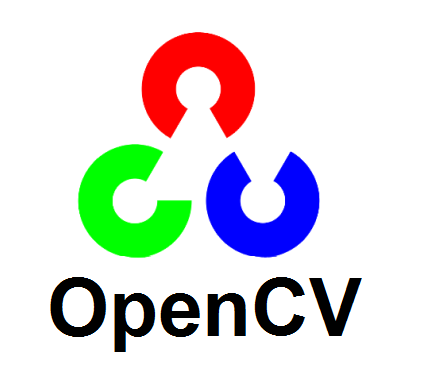
\includegraphics[width=0.6\textwidth]{opencv.png}
            \caption{Logo de Open Computer Vision}\label{fig:opencv}
        \end{figure}
        \normalfont
        OpenCV (Open Source Computer Vision Library) est une bibliothèque de logiciels open source de vision par ordinateur et d'apprentissage automatique. OpenCV a été développé pour fournir une infrastructure commune pour les applications de vision par ordinateur et  accélérer l'utilisation de la vision artificielle dans les produits commerciaux. OpenCV est un produit sous licence BSD, les entreprises peuvent donc facilement utiliser et  modifier  le code.
        
        La bibliothèque contient plus de 2500 algorithmes optimisés, y compris un ensemble complet d'algorithmes de vision par ordinateur et d'apprentissage automatique classiques et  de pointe. Ces algorithmes sont utilisés pour la détection et la reconnaissance de visages, l'identification d'objets, la classification du comportement humain dans les vidéos, le suivi de mouvement de caméra, le suivi d'objets en mouvement, l'extraction de modèles 3D d'objets, les nuages de points 3D à partir de caméras stéréo, Résolution d'images à travers des scènes, recherche d'images similaires dans des bases de données d'images, suppression des yeux rouges des images prises au flash, suivi des mouvements oculaires, détection de paysages, création de marqueurs à superposer avec la réalité augmentée, etc. OpenCV a une communauté de plus de 7 000 utilisateurs avec plus de 18 millions de téléchargements estimés. Cette bibliothèque est fréquemment utilisée par les entreprises, les groupes de recherche et les agences gouvernementales.

        \bfseries
        \item Tensorflow
        \begin{figure}[H]
            \centering
            
\includegraphics[width=0.6\textwidth]{tensorflow.png}
            \caption{Logo de Tensorflow}\label{fig:tensorflow}
        \end{figure}
        \normalfont
        TensorFlow est une plate-forme d'apprentissage automatique open source de bout en bout. TensorFlow est un système complet de gestion de tous les aspects des systèmes d'apprentissage automatique. Cependant, ce cours se concentre sur le développement et la formation de modèles d'apprentissage automatique à l'aide d'API TensorFlow spécifiques. 
        
        L'API TensorFlow est organisée de manière hiérarchique, avec des API de  niveau supérieur construites au-dessus des API de niveau inférieur. Les chercheurs en apprentissage automatique utilisent des API de bas niveau pour créer et explorer de nouveaux algorithmes d'apprentissage automatique. En utilisant tf.keras on peut définir et former des modèles d'apprentissage automatique  pour effectuer des prédictions. tf.keras est la version TensorFlow de l'API Keras open source.

        \bfseries
        \item Keras
        \begin{figure}[H]
            \centering
            
\includegraphics[width=0.6\textwidth]{keras.png}
            \caption{Logo de Keras}\label{fig:keras}
        \end{figure}
        \normalfont
        Keras est une API d'apprentissage en profondeur de haut niveau développée par Google pour la mise en œuvre de réseaux de neurones. Il est écrit en Python et est utilisé pour faciliter la mise en œuvre de réseaux de neurones. Il prend également en charge plusieurs calculs de  réseaux neuronaux principaux. 
        
        Keras est relativement facile à apprendre et à utiliser car il fournit une interface Python avec un haut niveau d'abstraction tout en offrant de multiples possibilités de backend à des fins de calcul. Cela rend Keras plus lent que les autres frameworks d'apprentissage en profondeur, mais très convivial pour les débutants.

        \bfseries
        \item Matplotlib
        \begin{figure}[H]
            \centering
            
\includegraphics[width=0.6\textwidth]{matplotlib.jpeg}
            \caption{Logo de Matplotlib}\label{fig:matplotlib}
        \end{figure}
        \normalfont
        Matplotlib est également l'une des bibliothèques les plus réussies et les plus utilisées, fournissant divers outils de visualisation de données en Python. 
        C'est l'une des bibliothèques de traçage les plus puissantes de Python. Il s'agit d'une bibliothèque multiplateforme qui fournit divers outils pour créer des tracés 2D à partir de données de liste ou de tableau en Python. 
        
        Matplotlib a été créé en 2003 dans le langage de programmation Python par Jean D. Hunter. Il utilise NumPy, une bibliothèque qui fournit des extensions mathématiques numériques pour Python. 
        
        Il expose également une API orientée objet qui vous permet d'étendre la possibilité de placer des graphiques statiques dans votre application à l'aide de divers kits d'outils d'interface graphique Python disponibles (Tkinter, PyQt, etc.). 
        Vous pouvez utiliser différents types de graphiques pour visualiser vos données et faciliter leur compréhension. En écrivant quelques lignes de code en Python, vous pouvez utiliser ces différents types de graphiques (scatter plots, histograms, bar charts, error charts, box charts, etc.).

        \bfseries
    \end{enumerate}
    \subsubsection{IDEs}
    \begin{enumerate}\bfseries
        \item Jupyter
        \begin{figure}[H]
            \centering
            
\includegraphics[width=0.6\textwidth]{jupyter.jpeg}
            \caption{Logo de Jupyter}\label{fig:jupyter}
        \end{figure}
        \normalfont
        Jupyter est une application Web permettant de programmer dans plus de 40 langages de programmation, dont Python, Julia, Ruby, R ou  Scala. Il s'agit d'un projet communautaire visant à développer des logiciels libres, des formats ouverts et des services pour l'informatique interactive. Jupyter est une évolution du projet IPython. Jupyter vous permet de créer des blocs-notes, des programmes contenant à la fois du texte  et du code Markdown. Ces cahiers sont utilisés  pour explorer et analyser des données en science des données.

        \bfseries
        \item Google Colab pro+
        \begin{figure}[H]
            \centering
            
\includegraphics[width=0.6\textwidth]{colab.png}
            \caption{Logo de Colab}\label{fig:colab}
        \end{figure}
        \normalfont
        Le service Google Colaboratory, ou Google Colab en abrégé, vous permet d'exécuter du code Python dans un navigateur Web dans ce que l'on appelle des "notebooks". Il est utilisé pour l'apprentissage en profondeur, le partage et le travail sur des projets de science des données avec d'autres.
        \begin{itemize}[label=$\bullet$]
            \item Cartes graphiques plus rapides
            
            Avec le Colab Pro/Pr, vous pouvez accéder à plus de ressources et  choisir des GPU plus rapides tels que NVIDIA Tesla T
            et NVIDIA Tesla P100 pour vos projets. En tant qu'utilisateur gratuit de Google Colab, je constate souvent que ma carte graphique ralentit et que ma RAM est faible. Lors de la création d'images ki (ki-générated images), le temps de traitement d'image des modèles Pro et Pro est environ 6 fois plus rapide que  le Colab gratuit. De quoi réserver au moins la version Colab Pro pour environ 10 euros par mois. 
            \item Durée d'exécution plus longue 
            
            La version Pro de Google Colab a également une durée d'exécution plus longue, gardant votre ordinateur portable connecté jusqu'à 24 heures, tandis que la version gratuite se déconnecte après seulement 12 heures. 
            L'avantage de la version Colab Pro ici est que l'instance continuera à s'exécuter  après la fermeture de la fenêtre du navigateur, mais dans les versions Free et Pro, la fermeture de la fenêtre mettra fin à l'instance. 
            \item Plus de RAM
            
            Les utilisateurs du modèle payant bénéficient également de plus de RAM. Vous devriez être satisfait de 16 Go pour le Colab gratuit, mais les utilisateurs Pro ont 32 Go et les utilisateurs Pro ont  52 Go de RAM. Les comptes payants sont particulièrement adaptés au traitement de grandes quantités de données.
        \end{itemize}
        
       
        \bfseries
    \end{enumerate}
    \subsubsection{HPC-MARWAN}
    \begin{figure}[H]
        \centering
        
\includegraphics[width=0.6\textwidth]{marwan-hpc.png}
        \caption{Logo de HPC-MARWAN}\label{fig:marwan-hpc}
    \end{figure}
    Le Centre National de la Recherche Scientifique et Technique met à la disposition de la communauté des chercheurs marocains une infrastructure de Calcul Haute Performance (HPC) accessible à distance.

    L'infrastructure compte 38 nœuds avec la capacité suivante:
    • 1672 cœurs de processeur (165 TFlops)
    • 396 To de stockage
    • 10,4 To de RAM
    • 4 GPU

    Les nœuds sont interconnectés via un réseau à faible latence à une bande passante de 100 Gbps, optimisant ainsi les performances de calcul parallèle. Un système de fichiers parallèle est implémenté pour faciliter un accès haute performance via des IOPS simultanées par plusieurs tâches d'une application parallèle.
    L'infrastructure est connectée à MARWAN via une liaison 5Gbps pour assurer des vitesses de transfert de données élevées depuis les universités et institutions connectées à MARWAN.

    \subsubsection*{SLURM Workload Manager}
    SLURM: Simple Linux Utility for Resource Management
    \begin{figure}[H]
        \centering
        
\includegraphics[width=0.6\textwidth]{slurm.png}
        \caption{Logo de SLURM}\label{fig:slurm}
    \end{figure}

    Slurm est un système de gestion de cluster et de planification des tâches open source, tolérant aux pannes et hautement évolutif pour les grands et petits clusters Linux. Slurm ne nécessite aucune modification du noyau pour son fonctionnement et est relativement autonome. En tant que gestionnaire de charge de travail de cluster, Slurm a trois fonctions clés. Premièrement, il alloue un accès exclusif et/ou non exclusif aux ressources (noeuds de calcul) aux utilisateurs pendant une certaine durée afin qu'ils puissent effectuer un travail. Deuxièmement, il fournit un cadre pour démarrer, exécuter et surveiller le travail (normalement un travail parallèle) sur l'ensemble des noeuds alloués. Enfin, il arbitre les conflits de ressources en gérant une file d'attente de travaux en attente. Des plug-ins facultatifs peuvent être utilisés pour la comptabilité, la réservation avancée, la planification des équipes (partage du temps pour les tâches parallèles), la planification des remplissages, la sélection des ressources optimisée pour la topologie, les limites de ressources par utilisateur ou compte bancaire et les algorithmes sophistiqués de hiérarchisation des tâches multifactorielles.

\section{Bases de données}
    Durant notre recherche pour une base de données convenable a notre projet on a trouver la liste des bases de données suivnates :
    \begin{table}[H]
        \centering
        \scriptsize
        \begin{tabularx}{\textwidth}{ |X|X|X|X|X|X|X|X| } 
            \hline
            \hfil Nom de base de données & \hfil Nombre des images & \hfil Pourcentage des images pédiatriques & \hfil Tranche d'âge & \hfil Étiquettes de recherche et de diagnostic & Étiquettes 
            \hfil spatiales & \hfil Taille de l'image & \hfil Statut d'accès\\ [1ex]
            \hline
            \hfil ChestX-Ray14 & \hfil 112120 & \hfil - & \hfil - & \hfil 14 & \hfil 0 & \hfil redimensionné 1024 x 1024 & \hfil - \\ 
            \hline
            \hfil PLCO & \hfil 185421 & \hfil - & \hfil - & \hfil 12 & \hfil 9 & \hfil taille originale & \hfil - \\ 
            \hline
            \hfil CheXpert & \hfil 224316 & \hfil 0\% & \hfil 18+ & \hfil 14 & \hfil 0 & \hfil taille originale & \hfil public \\ 
            \hline
            \hfil MIMIC-CXR & \hfil 371920 & \hfil - & \hfil - & \hfil 14 & \hfil 0 & \hfil taille originale & \hfil - \\ 
            \hline
            \hfil PadChest & \hfil 160868 & \hfil 34\% & \hfil - & \hfil 193 & \hfil 104 & \hfil taille originale & \hfil public \\
            \hline
            \hfil Kermany & \hfil 5856 & \hfil 100\% & \hfil 1-5 & \hfil 3 & \hfil 0 & \hfil taille originale & \hfil - \\ 
            \hline
            \hfil PERCH & \hfil 3587 & \hfil - & \hfil - & \hfil 5 & \hfil - & \hfil - & \hfil - \\
            \hline
            \hfil NIH-14 & \hfil 112120 & \hfil 46\% & \hfil 1–17 & \hfil 14 & \hfil 8 & \hfil 1024 x 1024 & \hfil - \\
            \hline
            \hfil RSNA & \hfil 30227 & \hfil 65\% & \hfil 1–17 & \hfil 3 & \hfil - & \hfil 1024 x 1024 & \hfil - \\
            \hline
            \hfil SIIM – ACR & \hfil 12047 & \hfil 19,53\% & \hfil 1–17 & \hfil 2 & \hfil - & \hfil 1024 x 1024 & \hfil - \\
            \hline
            \hfil NIAID & \hfil 6251 & \hfil 11\% & \hfil 1–17 & \hfil - & \hfil - & \hfil - & \hfil - \\
            \hline
            \hfil Shenzhen & \hfil 662 & \hfil 4,6\% & \hfil 2 mois - 17 anns & \hfil - & \hfil - & \hfil taille originale & \hfil - \\
            \hline
            \hfil Montgomery County & \hfil 138 & \hfil 12,3\% &  \hfil 4–17 & \hfil - & \hfil - & \hfil taille originale & \hfil - \\
            \hline
        \end{tabularx}
        \caption{Les bases données taitants le même phénomène}\label{table:all_dbs}
    \end{table}
    \subsection{CheXpertDB}\label{chexpertDB}
    Le choix de cette  jeu de données de CheXpert comme base du modèle de pré-entraînement est justifié devant :
    \begin{itemize}[label=$\bullet$]
        \item Sa grande taille  ( plus de 224,316  images recueillis rétrospectivement de l'hôpital de Stanford de 65,240 patients. ) 
        \item Son accessibilité au public sans aucune formation préalablement requise
        \item Le nombre important d’anomalies ciblées par l'étiquetage (14) avec une terminologie claire conforme au Glossaire des termes d'imagerie thoracique recommandé par ‘Fleischner Society’ de radiologie thoracique 
        \item l’existence de plusieurs applications sur un sous-ensemble ou  la totalité de ses données via des compétitions avec de haute performances publiées sur son site officiel et des scores d'experts auxquels les chercheurs peuvent comparer leurs modèles.
        

    \end{itemize}
    \subsection{XpediaDB}

\section*{Conclusion}